Accelerated material discovery involves searching over a large design space in an accelerated manner to find promising material(s) for an application of interest~\cite{ajayi2016rapid}.
For example, acceleration can be achieved by fast screening large search spaces by an autonomous guide or by down selecting from high-throughput data sampled from a large search spaces. 
One commonly encountered example of a material search space is a combinatorial discovery with the search space comprising of a grid with each dimension representing fractional composition of an element considered.
For example, in case of a ternary material, the grid is three dimensional with a total of \(10^3\) different materials to be studied~(for \(0.1\) compositional increments). 
A search space can be arbitrarily high-dimensional and its size increases exponentially with dimensions. 
Once a search space is selected~(or sampled), characteristic response(s) for an application of interest are collected. 
A response from a material can be scalar performance measure~(or a figure of merit) for a fixed stimuli~\cite{haber2014high,suram2015generating}, guided by expert knowledge about the material system or in general a spectrum collected over a range of the stimuli~\cite{hattrick2016perspective}. 
Spectral data forms a high-dimensional hypercube shown in Figure~\ref{fig:spectrahypercube} (adapted from~\cite{rajan2013informatics}) comprising characteristic responses from materials made via systematic variation of design variable (such as chemical composition in our case) to understand underlying property or mechanism of materials.
Spectral responses are high dimensional and often have convoluted features thus a multi-variate correlative study in a high dimensional search space is required to identify underlying phenomenon in the search space.
Previously, visual comparison of the spectra in a multi-variate fashion has been used to compute a physical parameter~\cite{de2008core,de19902p}. 
However, given the complicated and convoluted nature of the spectral data, extraction of physical parameters is ill-posed and mathematically intractable~\cite{suzuki2019automated}. 

In the first part of this thesis, we work with catalyst discovery experiments where the materials are characterized using a cyclic voltammetry~(CV). 
CV is an electrochemical technique with a pre-defined cyclic voltage sweep as a stimuli and current as output, giving rise to a spectral response for each material. 
CV has been used to extract thermodynamic~(over potential), kinetic~(rate constant) properties of materials~\cite{martin2016qualitative,rountree2014evaluation,haber2014high}. 
Figure \ref{fig:spectrahypercube} presents a spectral data view point and the goal of multi-variate study on CV spectrum. 
CV responses are closed loops with thermodynamic and kinetic information embedded into it in a convoluted manner. 
A multi-variate study on the spectral data would provide insight into \textit{when, where} and \textit{how} the spectra indicate changes for a given set of processing parameters.

\begin{figure}[h!]
    \centering
    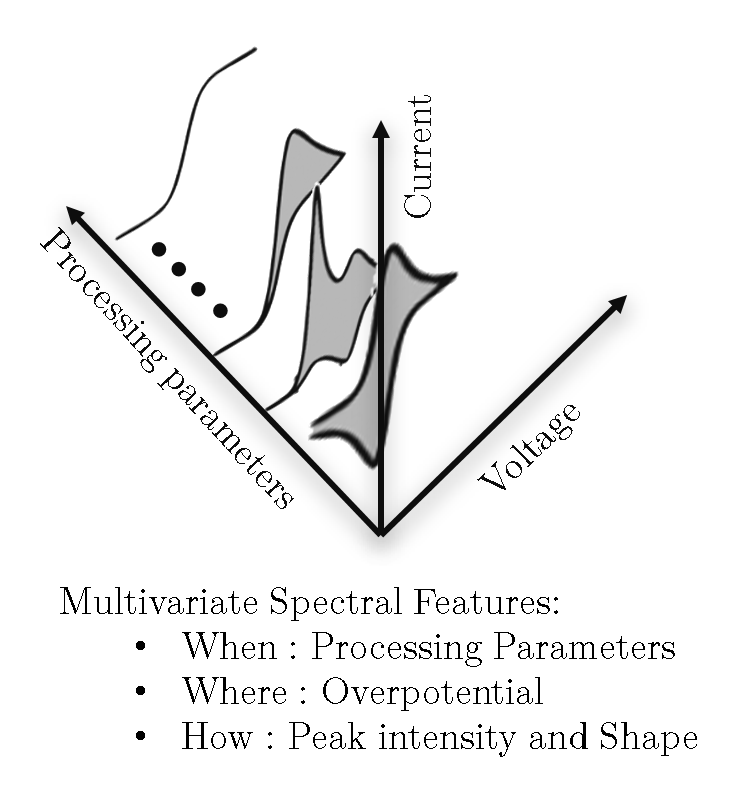
\includegraphics[width=0.45\columnwidth]{Chapter-1/figures/spectral_hypercube.png}
    \caption{Hypercube of data from a typical cyclic voltammetry characterization of a catalyst material (adapted from~\cite{rajan2013informatics}).}
    \label{fig:spectrahypercube}
\end{figure}


Data based models emerged as an ubiquitous tool for analyzing high-dimensional signals.
In the data-driven science paradigm, data is used as a resource to extract knowledge from a highly complex systems often with a goal of identifying new phenomena that is not possible with manual human reasoning with in a reasonable time frame~\cite{brunton2019data}.
We observe that data comes with two inherent properties: ~1) \textit{structure :} that assigns an arrangement~(often high dimensional) to each data point thereby capturing underlying governing characteristics of the sampled data that contribute to both local and global structure of dataset and ~2) \textit{stochasticity:} that assigns a probability to each data point that highlights relevance of a sampled data with in a context (for example an experiment). 
Encoding inherent properties of the data with a final goal of data analysis in mind is a key aspect often studied under the realm of \textit{representation}~\cite{bengio2013representation}. 
Structural representations are usually computed by assigning a metric space to the data, as it readily produces a notion of nearness and neighborhood that signifies an underlying local structure~\cite{mcinnes2018umap}. 
Other representations that encode a structure include graphs and simplicial sets for example. 
Representations that encode stochasticity of data points typically use a distribution such as Gaussian~\cite{gardner2015bayesian,gavaghan2018use} and Poisson~\cite{flory1940molecular}.


We identify the following challenges from a representation point of view for data-driven material design and discovery:
\begin{itemize}
    \item {\textbf{Structure and Continuous data space: }Materials have an inherent connectivity as depicted in a periodic table for example, where each element is assigned an arrangement based on atomic number, electronic configuration and other recurring chemical properties~\cite{periodictable}. In general, this is true for data sampled from experiments or simulations over a property design space. Enforcing continuity constraints into data analysis of characteristic responses is a key challenge to understand the structure of the dataset~\cite{lebras2011constraint}}
    \item {\textbf{Stochasticity and Prior knowledge exploitation:} Responses from experiments involving synthesis and characterization can be assigned a probability of occurrence that is governed by underlying material characteristics such as a mechanism, crystal structure etc~\cite{hull2018stochasticity}. Encoding prior knowledge about stochasticity of a given characterization or synthesis of a material can greatly improve output of a data analysis and better guide data sampling.  For example, X-ray diffraction data analysis has greatly benefited from a representation that decodes each signal as a superposition of few basis patterns each representing a possible phase~\cite{Kusne2015HighthroughputDO,hattrick2016perspective}. For each signal with potential mixed phases, each pure phase is assigned a possibility of presence based on observed relative peak intensity giving rise to a stochastic representation used for deducing a phase mapping~\cite{gomes2019crystal,stanev2018unsupervised}}
\end{itemize}


